\documentclass{article}

\usepackage{arxiv}

\usepackage[utf8]{inputenc} % allow utf-8 input
\usepackage[T1]{fontenc}    % use 8-bit T1 fonts
\usepackage{hyperref}       % hyperlinks
\usepackage{url}            % simple URL typesetting
\usepackage{booktabs}       % professional-quality tables
\usepackage{amsfonts}       % blackboard math symbols
\usepackage{nicefrac}       % compact symbols for 1/2, etc.
\usepackage{microtype}      % microtypography
\usepackage{lipsum}
\usepackage{graphicx}

\title{Ownership dynamics, risk and regulation in Chinese banking: New Evidence}

\author{
    Veronica Zhang
    \thanks{The authors gratefully acknowledge Professor John Turner and Dr Clive
Walker for their insight comments.}
   \\
    Management School, Queen's University Belfast \\
   \\
  \texttt{} \\
   \And
    Lisa Sheenan
   \\
    Management School, Queen's University Belfast \\
   \\
  \texttt{} \\
   \And
    Barry Quinn
   \\
    Management School, Queen's University Belfast \\
   \\
  \texttt{} \\
  }

\usepackage{color}
\usepackage{fancyvrb}
\newcommand{\VerbBar}{|}
\newcommand{\VERB}{\Verb[commandchars=\\\{\}]}
\DefineVerbatimEnvironment{Highlighting}{Verbatim}{commandchars=\\\{\}}
% Add ',fontsize=\small' for more characters per line
\usepackage{framed}
\definecolor{shadecolor}{RGB}{248,248,248}
\newenvironment{Shaded}{\begin{snugshade}}{\end{snugshade}}
\newcommand{\AlertTok}[1]{\textcolor[rgb]{0.94,0.16,0.16}{#1}}
\newcommand{\AnnotationTok}[1]{\textcolor[rgb]{0.56,0.35,0.01}{\textbf{\textit{#1}}}}
\newcommand{\AttributeTok}[1]{\textcolor[rgb]{0.77,0.63,0.00}{#1}}
\newcommand{\BaseNTok}[1]{\textcolor[rgb]{0.00,0.00,0.81}{#1}}
\newcommand{\BuiltInTok}[1]{#1}
\newcommand{\CharTok}[1]{\textcolor[rgb]{0.31,0.60,0.02}{#1}}
\newcommand{\CommentTok}[1]{\textcolor[rgb]{0.56,0.35,0.01}{\textit{#1}}}
\newcommand{\CommentVarTok}[1]{\textcolor[rgb]{0.56,0.35,0.01}{\textbf{\textit{#1}}}}
\newcommand{\ConstantTok}[1]{\textcolor[rgb]{0.00,0.00,0.00}{#1}}
\newcommand{\ControlFlowTok}[1]{\textcolor[rgb]{0.13,0.29,0.53}{\textbf{#1}}}
\newcommand{\DataTypeTok}[1]{\textcolor[rgb]{0.13,0.29,0.53}{#1}}
\newcommand{\DecValTok}[1]{\textcolor[rgb]{0.00,0.00,0.81}{#1}}
\newcommand{\DocumentationTok}[1]{\textcolor[rgb]{0.56,0.35,0.01}{\textbf{\textit{#1}}}}
\newcommand{\ErrorTok}[1]{\textcolor[rgb]{0.64,0.00,0.00}{\textbf{#1}}}
\newcommand{\ExtensionTok}[1]{#1}
\newcommand{\FloatTok}[1]{\textcolor[rgb]{0.00,0.00,0.81}{#1}}
\newcommand{\FunctionTok}[1]{\textcolor[rgb]{0.00,0.00,0.00}{#1}}
\newcommand{\ImportTok}[1]{#1}
\newcommand{\InformationTok}[1]{\textcolor[rgb]{0.56,0.35,0.01}{\textbf{\textit{#1}}}}
\newcommand{\KeywordTok}[1]{\textcolor[rgb]{0.13,0.29,0.53}{\textbf{#1}}}
\newcommand{\NormalTok}[1]{#1}
\newcommand{\OperatorTok}[1]{\textcolor[rgb]{0.81,0.36,0.00}{\textbf{#1}}}
\newcommand{\OtherTok}[1]{\textcolor[rgb]{0.56,0.35,0.01}{#1}}
\newcommand{\PreprocessorTok}[1]{\textcolor[rgb]{0.56,0.35,0.01}{\textit{#1}}}
\newcommand{\RegionMarkerTok}[1]{#1}
\newcommand{\SpecialCharTok}[1]{\textcolor[rgb]{0.00,0.00,0.00}{#1}}
\newcommand{\SpecialStringTok}[1]{\textcolor[rgb]{0.31,0.60,0.02}{#1}}
\newcommand{\StringTok}[1]{\textcolor[rgb]{0.31,0.60,0.02}{#1}}
\newcommand{\VariableTok}[1]{\textcolor[rgb]{0.00,0.00,0.00}{#1}}
\newcommand{\VerbatimStringTok}[1]{\textcolor[rgb]{0.31,0.60,0.02}{#1}}
\newcommand{\WarningTok}[1]{\textcolor[rgb]{0.56,0.35,0.01}{\textbf{\textit{#1}}}}

% Pandoc citation processing

\begin{document}
\maketitle

\def\tightlist{}


\begin{abstract}
Enter the text of your abstract here.
\end{abstract}

\keywords{
    financial institutions
   \and
    Industrial organisation
  }

\hypertarget{introduction}{%
\section{Introduction}\label{introduction}}

\label{sec:intro}

The relationship between capital buffers and bank risk-taking has long
attracted academic attention, ({\textbf{???}}; Demirgüç-Kunt and Kane
2002; Keeley 1990). The implementation of Basel Accords also lead to
work focusing on the effects of capital regulation on bank behaviour, in
particular on the impact of capital adequacy requirements on bank
risk-taking behaviour. The 2007-2009 global financial crisis uncovered
structural weaknesses in capital regulations which were implemented
before the crisis. After the crisis, the Basel Committee on Banking
Regulation and Supervision (BCBS) developed a consolidated framework
(Basel III) for more stringent capital adequacy regulations and
liquidity assessment, in recognition of the need for banks to be subject
to more stringent capital regulations. Following the goals set by the
BCBS, member countries, including China, have established legislation
and regulatory frameworks. While regulatory consensus has been reached
focusing on capital buffers, there is continued academic debate about
what effect capital requirements could have on bank risk-taking
(Chiaramonte and Casu 2017; Demirguc-Kunt, Detragiache, and Merrouche
2013; Roulet 2018)

China's banking sector plays an essential role in the country's economic
development. It underwent fundamental reform in 1978, as an integrate
part of China's overall economic reform. Since 2001, when China got
accession to the World Trade Organization (WTO), the reform of China's
banking system has stepped up its pace and the whole banking sector has
been dramatically reshaped. The reform has transformed Chinese banks
into market-oriented enterprises, changed their ownership structure,
established modern corporate governance mechanisms, and introduced
legislation and regulatory framework. Since 2010, improvements and
refinements have continued in China's banking sector as part of an
advanced stage of the reform. China's financial authority fully accepted
the Basel III framework and began its implementation in 2013. A rich
body of literature focusing on the previous stages of the reform
assesses the relationship between capital requirements and Chinese
banks' performance and risk-taking (Lee and Chih 2013; Pessarossi and
Weill 2015; Tan and Floros 2013). The objective of this paper is to
analyze the impact of capital requirements on Chinese bank risk-taking
following the 2007-2009 global financial crisis using the risk-based
capital definition of the Basel III framework.

In this paper, we extend existing empirical work studying the impact of
capital requirements on bank credit risk-taking by incorporating the
interaction between capital regulation and ownership structure.
Financial theories suggest that capital regulations impact banks'
risk-taking due to the effect of the regulation on shareholders'
incentives. (Allen, Carletti, and Marquez 2011; Demirgüç-Kunt and Kane
2002) (Demirgüç-Kunt and Kane, 2002, Allen et al., 2011) Empirical
studies support those theories. Nevertheless, empirical studies find
mixed results including negative association {[}RN24,RN75{]} (Berger and
Bouwman, 2013, Tan and Floros, 2013), positive association {[}RN27{]}
(Bichsel and Blum, 2004) and nonlinear relationships (Calem and Rob
1999) between capital regulation and bank risk-taking. Agency theory
suggests that corporate risk-taking is influenced by ownership structure
depending on the power of shareholder control. (Jensen and Meckling
1976, @RN4) Therefore, these theoretical keystones provide the
foundation for us to examine the effect of capital regulation on bank
risk-taking and how this interacts with ownership structure in
determining risk-taking.

This paper provides empirical evidence using forensically analysed data
on 231 China's commercial banks over the period 2010-2019. To perform
our analysis, we also hand collect the ownership structure information
of these 231 Chinese commercial banks and classify them into 5
categories of ownership identities: State-owned (Big Six and other than
Big Six), Local government-holding, Joint-stock, Foreign joint-stock,
and Foreign-owned banks. (Table 1) We regress both regulatory capital
requirements from the Basel III framework and ownership identities on
bank credit risk-taking proxies, respectively. We employ banks'
Non-performing Loans (NPL) ratios and Loan Loss Reserves (LLR) ratios to
reflect the level of banks' credit risk-taking. We also examine the
actual impact of Basel III capital regulation on credit risk-taking
incorporating the interaction between capital regulation and ownership
structure.

Our key findings are as follows. First, credit risk is generally lower
in banks that have higher regulatory capital. This finding is consistent
with the theory suggesting regulatory capital acts as a buffer to resist
economic shocks and lower banks' risk-taking incentives (Demirguc-Kunt,
Detragiache, and Merrouche 2013, @RN64). This finding also supports the
empirical studies of Chinese banks conducted by Tan and Floros (2013)
and Lee, Ning, and Lee (2015).

Second, state-owned banks in general have higher credit risk compared to
foreign-owned banks and other ownership identities. This finding is
consistent with the results of Zhu and Yang (2016) which examines
risk-taking of state-owned banks and foreign banks. This finding also,
to some extent, backs up the empirical results of Laeven and Levine
(2009) which finds banks with large owners who have significant cash
flow rights take higher credit risk. During the financial reform, the
state-shareholder in Chinese banks has transformed from a state-bureau
(e.g., the Finance Ministry) to a state-corporation (e.g., Central
Huijin Investment Co.) with modern corporate governance mechanisms. The
state-shareholder has become a shareholder with \emph{highly
concentrated control rights and significant cash flow rights}. Due to
this fact, our finding can be considered consistent with the agency
theory that concentrated ownership and powerful shareholders suggest
higher corporate risk-taking(Saunders, Strock, and Travlos 1990; Stulz
2005). This finding also supports the social view of the theory of state
ownership of banks that state-owned banks would undertake credit
projects which might not be financially profitable(Stiglitz 1993).

Third, the actual impact of Basel III capital regulation on credit
risk-taking can be influenced, to some extent, by ownership structure.
For example, the results suggest that in government-holding banks, the
negative effect of capital regulation on credit risk-taking can be
enhanced by its ownership identity when there is no shareholder with
significant power to increase risk-taking incentives.

This paper contributes to the literature in several ways. First, this
study assesses the impact of risk-based capital regulation on Chinese
bank credit risk-taking following the global financial crisis, using the
definition of capital from Basel III framework. It has been 10 years
since the BCBS first released Basel III framework in 2010. The Chair of
the BCBS stated that evaluating the regulation effects is part of the
BCBS post-crisis reform in the current macroeconomic environment. In
addition, China's banking industry achieved extensive transformation
before 2010 and the Chinese case provides uniqueness in terms of
ownership structure.

Second, our study bridges the research gap by incorporating the
interaction between ownership structure and capital regulation while
examining the impact of Basel III capital requirements on bank credit
risk-taking. Only a small number of existing studies evaluate the joint
effects of ownership structure and bank regulations on bank risk-taking,
such as Laeven and Levine (2009) 2009. Pessarossi and Weill (2015) test
the impact of the interaction between capital regulation and ownership
structure on cost efficiency of Chinese banks. To the best of our
knowledge, this is the first study to assess how Basel III regulation
and ownership structure jointly shape Chinese bank credit risk-taking
following the global financial crisis.

Third, we analyse a bespoke dataset of 231 Chinese commercial banks over
a relatively long period (2010-2019) to study China's banking sector.
These 231 banks account for over 80\% of China's banking sector in terms
of total assets. Apart from employing the data provided by the SNL
database, we hand collected any missing values from the original annual
reports of individual banks, which makes our data set extremely
comprehensive.

The remainder of this paper is organised as follows. Section II reviews
related literature, develops the testable predictions, as well as a
brief introduction of the evolution of ownership structure of commercial
banks in China. Section III presents the data set and the empirical
model including the variables considered in our analysis. The empirical
results are presented in section IV. And section V concludes.

\hypertarget{literature}{%
\section{Literature}\label{literature}}

As a member of the G20 and the Basel Committee on Banking Supervision,
China has been fully supporting and participating in the global
regulatory reform following the Great Financial Crisis of 2007-2009. In
June 2012, The China Banking Regulatory Commission (CBRC) issued the
regulation \emph{Commercial Bank Capital Management Measure (Trial)},
which means that the Basel III framework was adopted and incorporated
into the banking regulatory framework in China. The relationship between
macro and micro prudential regulations has a hierarchical structure.
Borio (2003) argue that the objectives of macro-prudential regulation
subsume the rationales of the micro-prudential approach. The Basel III
Framework is a macro-prudential framework based on Basel II framework (a
micro-prudential framework). Through examining the relation between
credit risk/solvency risk and Basel III, the impact of this
macro-prudential oriented framework can be assessed from the
institutional angle.

\hypertarget{bank-capital-and-risk}{%
\subsection{Bank capital and risk}\label{bank-capital-and-risk}}

Empirical literature and financial theories provide mixed views
regarding the impact of bank capital on risk-taking and bank stability.
The Basel framework, centered with capital regulation, is designed to
reduce bank risk and enhance bank resilience. Anginer and Demirguc-Kunt
(2014) support this view that bank capital acts as a buffer in absorbing
economic shocks and strengthens systemic stability. Demirguc-Kunt,
Detragiache, and Merrouche (2013) find that a strong capital position
helps banks resist earning shocks and have higher probability to survive
the crisis. They also find evidence to advocate higher quality capital,
i.e., Tier 1 capital, in the regulatory capital requirements. A lot of
theories underline that risk-based capital, more effective than interest
rate ceilings, boosts banks' ``franchise value'', improve borrowers
screening, and lower banks' excessive risk-taking incentives {[}Allen,
Carletti, and Marquez (2011);RN64;RN67{]}. Other theories emphasize a
moral hazard perspective, arguing effective regulatory capitalization
may offset the excessive risk-taking incentives created by deposit
insurance (Keeley 1990; Demirgüç-Kunt and Kane 2002). In terms of
Chinese commercial banks, (Tan and Floros 2013) find a significant
negative relationship between bank capital and risk. ({\textbf{???}})
report that bank capital is negatively related to NPL and support
theories with the moral hazard view.

Contrariwise, other research posits that greater capital regulations may
induce higher bank risk. Cooper and Ross (2002) extend the research of
Diamond and Dybvig (1983), stating that the existence of deposit
insurance weaken the depositors' incentive to monitor banks and causes
them to engage in excessive risk-taking activities. Blum (1999) suggests
that banks may have higher incentives to raise risk due to the binding
capital adequacy requirements. Calem and Rob (1999) find a U-shaped
relationship between bank capital position and risk. The risk-taking
first decreases with the increase of bank capital; then it increases as
bank capital increases on its high level. They also argue that the
increase in capital adequacy requirements induces banks to take
additional portfolio risk even if they are well-capitalized. For Chinese
banking data, Lee and Chih (2013) find that the negative relationship
between capital and risk only exists in the sub-sample of small banks
and is not found in the sub-sample of large banks. We test the following
two hypotheses regarding the impact of regulatory capital requirements
on bank credit risk:

\textbf{Hypothesis 1a:} \emph{There is a negative relationship between
regulatory capital and credit risk.}

\textbf{Hypothesis 1b:} \emph{There is a positive relationship between
regulatory capital and credit risk.}

\hypertarget{ownership-structure-and-risk}{%
\subsection{Ownership structure and
risk}\label{ownership-structure-and-risk}}

Agency theory posits that corporate governance affects corporate
risk-taking in sourcing outside financing and in the choice of
value-enhancing projects because the private benefit of corporate
control comes at the expense of the firm's outside investors (Jensen and
Meckling 1976). As one of the most important approaches to corporate
governance, the legal investor protection (shareholder rights) approach
suggests that corporate risk-taking is influenced by shareholder rights.
Agency theory literature provides the results of both positive and
negative links between shareholder rights and firms' risk-taking. Amihud
and Lev (1981) and Hirshleifer and Thakor (1992) argue that in firms
where managers have high levels of discretion, managers have the motive
to engage their firms in conservative investment projects such as
conglomerate mergers and low net present value (NPV) projects, in order
to protect their careers or build their professional reputation. Based
on this view, better investor protection may constrain the managers'
excessive control rights in firms, and may result in higher corporate
risk-taking behaviour. John, Litov, and Yeung (2008) conduct a
cross-country study and support this view. They find a positive
relationship between investor protection and corporate risk-taking.

This school of thought suggests that investor protection is negatively
related to corporate risk-taking. Burkart, Panunzi, and Shleifer (2003)
argue that strong investor protection gives managers latitude to divert
company resources within their compensation packages. Therefore, it
would be optimal for the firm founders to sell the equity and hire
professionals to manage the company. According to this view, strong
legal protection, in fact, leads to a scenario of no controlling
shareholding in firms; and induces managers to take more conservative
actions in choosing investment in order to protect their private
benefit. The model provided by Burkart, Panunzi, and Shleifer (2003)
predicts that there is a negative relationship between legal investor
protection and ownership concentration which is another popular approach
to corporate governance.

Ownership concentrated in large investors with significant control
rights and significant cash flow rights is another common approach to
corporate governance (Laeven and Levine 2009). La Porta, Florencio, and
Shleifer (1999) suggest that corporations with dominant owners are more
commonly seen around the world, compared to widely held firms.
Controlling shareholders with strong incentives of monitoring inside
managers and maximizing firms' expected profits, execute their control
rights and cash flow rights mainly through the \emph{pyramid} corporate
setting (La Porta, Florencio, and Shleifer 1999; Shleifer and Vishny
1986). Agency models of large investors suggest a positive relationship
between ownership concentration and corporate risk-taking. Saunders,
Strock, and Travlos (1990) argue that stockholder controlled banks have
more intention to take higher risks than banks controlled by managers.
Stulz (2005) suggests that highly concentrated ownership decreases risk
aversion of managers inside the firms. Laeven and Levine (2009) provide
empirical evidence supporting banks with concentrated shareholding
generally have higher risk.

\hypertarget{state-ownership}{%
\subsection{State ownership}\label{state-ownership}}

State ownership is regarded as one of the special corporate
arrangements. From a corporate governance perspective, state firms are
defined as being ``controlled by the public; and the de facto control
rights usually belong to bureaucrat shareholders with highly
concentrated control rights and no significant cash flow rights''
(Shleifer and Vishny 1997). According to this view, state shareholders
can be considered as a special form of large investors with highly
concentrated control rights and lack of cash flow rights.

There are two alternative theories in the literature regarding the state
ownership in banks; the social view and the political view. The social
view, based on the economic theory of institutions, suggests that state
ownership is a form of government intervention which addresses market
failures and improves market functions and economic performance
(Stiglitz 1993). According to this view, state-owned banks may finance
those projects which might not be profitable but might have a high value
of social welfare. Therefore, state-owned banks may have poorer
performance in terms of profitability along with higher default risk
compared to their counterparties in the private sector. In contrast, the
political view claims that state ownership creates sources of political
benefits for politicians rather than social welfare. For example,
excessive employment of state firms only benefits those who support
government politically (Shleifer and Vishny 1994). Shleifer and Vishny
(1997) suggests that state-owned firms are inefficient because the state
shareholders, with highly concentrated control rights and no cash flow
rights, only maximize their political goals which may jeopardize social
welfare.

There is an extant literature examines the impact of state ownership of
banks, from both a macroeconomic angle and the perspective of individual
banks, mostly on economic growth and bank performance. Andrianova,
Demetriades, and Shortland (2012) find that state ownership of banks
improves countries' long-run economic growth. However, La Porta,
Florencio, and Shleifer (2002) find that higher government ownership is
related to lower economic growth. Beck and Levine (2002) find no
supporting evidence for either the social view or the political view. At
the individual bank level, studies tend to focus on bank performance
under different ownership structures. Many studies report that
state-owned banks are less efficient than private-owned banks. For
example, Beck, Demirgüç-Kunt, and Maksimovic (2004)\} argue that state
ownership intensifies bank concentration and restrains market
competition. Berger et al. (2005) and Iannotta, Nocera, and Sironi
(2007) find that state-owned banks have lower profitability and poor
long-term performance.

Ownership structure of banks in China's financial markets has attracted
academic attention following China's accession to the WTO in 2001. Many
studies focusing on bank efficiency report that state-owned banks
exhibit lower efficiency compared to joint-stock banks and foreign banks
(Berger, Hasan, and Zhou 2009; Fungáčová, Pessarossi, and Weill 2013).
Several papers focus on ownership structure and bank risk. Tan and
Floros (2013) argue that state-owned banks have higher volume of
non-performing loans and lower profitability. Zhu and Yang (2016) report
that state-owned banks take higher risk than foreign banks in China.

\hypertarget{the-evolution-of-ownership-structure-of-commercial-banks-in-china}{%
\subsection{The evolution of ownership structure of commercial banks in
China}\label{the-evolution-of-ownership-structure-of-commercial-banks-in-china}}

The dramatic changes regarding the ownership structure of commercial
banks in China are an essential part of every stage of China's financial
reform. The four largest state-owned banks were founded during the first
stage of the financial reform (1978-early 1990s), along with other
national banks. These big banks were owned by the Finance Ministry and
state-owned enterprises. The lower level of financial institutions,
known as city credit cooperatives, were controlled by the local Bureau
of Finance and foreign banks were operating in Special Economic Zones
(Berger, Hasan, and Zhou 2009). During the second stage (early
1990s-2001), most of the `policy-lending' business of the largest four
state-owned banks was released to three policy banks founded during this
period. Private enterprises and individuals began entering different
levels of financial institutions as shareholders. Local Bureaus of
Finance began to exit city banks by transferring their shareholding to
local business enterprises. The biggest change to the ownership
structure happened at the third stage of the financial reform
(2001-2010). An investment enterprise, Central Huijin Investment
Ltd.~(hereafter CH), was established by the state government acting as a
designated shareholder of those state-owned banks, in order to fulfil
the corporate governance requirements set by laws and regulations.
Direct government shareholding has sharply decreased. Foreign financial
institutions such as RBS Group and Bank of America invested in all
levels of Chinese banks including state-owned banks, national banks and
city banks, as strategic investors. The majority of state-owned banks
and several city banks went public at this stage, introducing more
diversified shareholders. After 2010, more detailed improvements
happened regarding ownership structure. Private-owned banks were
established. Local government shareholders become minority shareholders
in city banks. Over 50\% of shareholding in city banks and over 87\% of
shareholding in rural commercial banks had become private enterprises by
2017. In total 50 commercial banks were listed by 2019.

Based on the above discussion, we test the following two hypotheses
regarding the relationship between ownership structure and bank credit
risk in China's banking sector:

\textbf{Hypothesis 2a:} \emph{state-owned banks have higher credit risk
compared to other type of banks.}

\textbf{Hypothesis 2b:} \emph{state-owned banks do not have higher
credit risk compared to other type of banks.}

\hypertarget{ownership-structure-and-regulation}{%
\subsection{Ownership structure and
regulation}\label{ownership-structure-and-regulation}}

Financial theories suggest that banking regulations impact banks'
risk-taking by influencing shareholders' incentives (Allen, Carletti,
and Marquez 2011; Demirgüç-Kunt and Kane 2002). Corporate governance
theories suggest that ownership structure affects corporate risk-taking
through shareholder control rights on corporate decision-making (Jensen
and Meckling 1976, @RN4). Few studies on bank risk and regulation take
account of the interaction between regulation and ownership structure.
However, Koehn and Santomero (1980) argue that bank owners would
compensate their potential expected utility loss by allocating assets to
riskier portfolios when facing more stringent capital regulation. This
means that the effects of bank regulation on credit risk are manifested
through bank owners' incentives and power. Boyd and Hakenes (2008) set
up models examining the relation between bank risk-taking and bank
regulations under the circumstances of different ownership structure.
They claim that banks' incentives for taking excessive risk
(risk-shifting) and bank managers' looting, in response to bank
regulations, are affected by ownership structure. Laeven and Levine
(2009) further the empirical research of bank risk, regulation, and
ownership structure by examining cross-country data. They find that the
stringency of regulatory oversight can be dampened by ownership with
large control rights and cash flow rights. Concerning empirical studies
of commercial banks in China, Pessarossi and Weill (2015) suggest that
the effects of capital requirements on commercial banks may vary
depending on the individual banks' ownership structure. Thus, based on
financial theories and corporate governance theories, we examine whether
or not bank regulation and ownership structure jointly impact on bank
credit risk:

\textbf{Hypothesis 3a:} \emph{the impact of bank regulation on credit
risk depends on ownership structure.}

\textbf{Hypothesis 3b:} \emph{the impact of bank regulation on credit
risk does not depend on ownership structure.}

\hypertarget{data-and-forensic-accounting-anaysis}{%
\subsection{Data and forensic accounting
anaysis}\label{data-and-forensic-accounting-anaysis}}

This study uses annual data for 231 commercial banks in China, for the
period 2010-2019, providing a total of 2,310 observations. The
categories of sample financial institutions of the banking sector and
their ownership structure are listed in Table 1.

\begin{center}
    {Insert Table 1 Here}
\end{center}

\hypertarget{introduction-1}{%
\section{Introduction}\label{introduction-1}}

\lipsum[2]
\lipsum[3]

\hypertarget{headings-first-level}{%
\section{Headings: first level}\label{headings-first-level}}

\lipsum[4] See Section \ref{sec:headings}.

\hypertarget{headings-second-level}{%
\subsection{Headings: second level}\label{headings-second-level}}

\lipsum[5]

\[
\xi _{ij}(t)=P(x_{t}=i,x_{t+1}=j|y,v,w;\theta)= {\frac {\alpha _{i}(t)a^{w_t}_{ij}\beta _{j}(t+1)b^{v_{t+1}}_{j}(y_{t+1})}{\sum _{i=1}^{N} \sum _{j=1}^{N} \alpha _{i}(t)a^{w_t}_{ij}\beta _{j}(t+1)b^{v_{t+1}}_{j}(y_{t+1})}}
\]

\hypertarget{headings-third-level}{%
\subsubsection{Headings: third level}\label{headings-third-level}}

\lipsum[6]

\paragraph{Paragraph}
\lipsum[7]

\hypertarget{examples-of-citations-figures-tables-references}{%
\section{Examples of citations, figures, tables,
references}\label{examples-of-citations-figures-tables-references}}

\label{sec:others}

\lipsum[8] some text ({\textbf{???}}; {\textbf{???}}) and see
({\textbf{???}}).

The documentation for \verb+natbib+ may be found at

\begin{center}
  \url{http://mirrors.ctan.org/macros/latex/contrib/natbib/natnotes.pdf}
\end{center}

Of note is the command \verb+\citet+, which produces citations
appropriate for use in inline text. For example,

\begin{verbatim}
   @hasselmo} investigated\dots
\end{verbatim}

produces

\begin{quote}
  Hasselmo, et al.\ (1995) investigated\dots
\end{quote}

\begin{center}
  \url{https://www.ctan.org/pkg/booktabs}
\end{center}

\hypertarget{figures}{%
\subsection{Figures}\label{figures}}

\lipsum[10]

See Figure \ref{fig:fig1}. Here is how you add footnotes. {[}\^{}Sample
of the first footnote.{]}

\lipsum[11]

\begin{figure}
  \centering
  \fbox{\rule[-.5cm]{4cm}{4cm} \rule[-.5cm]{4cm}{0cm}}
  \caption{Sample figure caption.}
  \label{fig:fig1}
\end{figure}

\begin{Shaded}
\begin{Highlighting}[]
\KeywordTok{plot}\NormalTok{(mtcars}\OperatorTok{$}\NormalTok{mpg)}
\end{Highlighting}
\end{Shaded}

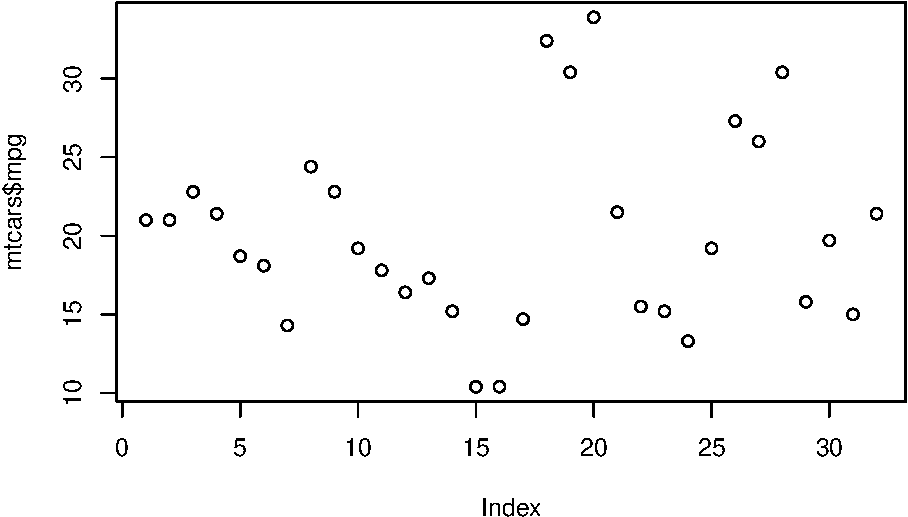
\includegraphics{preprint_files/figure-latex/unnamed-chunk-1-1.pdf}

\hypertarget{tables}{%
\subsection{Tables}\label{tables}}

\lipsum[12]

See awesome Table\textasciitilde{}\ref{tab:table}.

\begin{table}
 \caption{Sample table title}
  \centering
  \begin{tabular}{lll}
    \toprule
    \multicolumn{2}{c}{Part}                   \\
    \cmidrule(r){1-2}
    Name     & Description     & Size ($\mu$m) \\
    \midrule
    Dendrite & Input terminal  & $\sim$100     \\
    Axon     & Output terminal & $\sim$10      \\
    Soma     & Cell body       & up to $10^6$  \\
    \bottomrule
  \end{tabular}
  \label{tab:table}
\end{table}

\hypertarget{appendix}{%
\section{Appendix}\label{appendix}}

\hypertarget{a1.-definitions-of-the-basel-accords}{%
\subsection*{A1. Definitions of the Basel
Accords}\label{a1.-definitions-of-the-basel-accords}}
\addcontentsline{toc}{subsection}{A1. Definitions of the Basel Accords}

\hypertarget{refs}{}
\leavevmode\hypertarget{ref-RN15}{}%
Allen, Franklin, Elena Carletti, and Robert Marquez. 2011. ``Credit
Market Competition and Capital Regulation.'' Journal Article. \emph{The
Review of Financial Studies} 24 (4): 983--1018.
\url{http://www.jstor.org.queens.ezp1.qub.ac.uk/stable/20869263}.

\leavevmode\hypertarget{ref-RN16}{}%
Amihud, Yakov, and Baruch Lev. 1981. ``Risk Reduction as a Managerial
Motive for Conglomerate Mergers.'' Journal Article. \emph{The Bell
Journal of Economics} 12 (2): 605--17.
\url{https://doi.org/10.2307/3003575}.

\leavevmode\hypertarget{ref-RN17}{}%
Andrianova, Svetlana, Panicos Demetriades, and Anja Shortland. 2012.
``Government Ownership of Banks, Institutions and Economic Growth.''
Journal Article. \emph{Economica} 79 (315): 449--69.
\url{http://www.jstor.org/stable/23274805}.

\leavevmode\hypertarget{ref-RN18}{}%
Anginer, Deniz, and Asli Demirguc-Kunt. 2014. ``Bank Capital and
Systemic Stability.'' Journal Article. \emph{Policy Research Working
Papers} 6948 (June 2014): 42.
\url{https://doi.org/doi:10.1596/1813-9450-6948}.

\leavevmode\hypertarget{ref-RN22}{}%
Beck, Thorsten, Asli Demirgüç-Kunt, and Vojislav Maksimovic. 2004.
``Bank Competition and Access to Finance: International Evidence.''
Journal Article. \emph{Journal of Money, Credit and Banking} 36 (3):
627--48.
\url{http://www.jstor.org.queens.ezp1.qub.ac.uk/stable/3838958}.

\leavevmode\hypertarget{ref-RN23}{}%
Beck, Thorsten, and Ross Levine. 2002. ``Industry Growth and Capital
Allocation:: Does Having a Market- or Bank-Based System Matter?''
Journal Article. \emph{Journal of Financial Economics} 64 (2): 147--80.
\url{https://doi.org/https://doi.org/10.1016/S0304-405X(02)00074-0}.

\leavevmode\hypertarget{ref-RN25}{}%
Berger, Allen N., George R. G. Clarke, Robert Cull, Leora Klapper, and
Gregory F. Udell. 2005. ``Corporate Governance and Bank Performance: A
Joint Analysis of the Static, Selection, and Dynamic Effects of
Domestic, Foreign, and State Ownership.'' Journal Article. \emph{Journal
of Banking \& Finance} 29 (8): 2179--2221.
\url{https://doi.org/https://doi.org/10.1016/j.jbankfin.2005.03.013}.

\leavevmode\hypertarget{ref-RN26}{}%
Berger, Allen N., Iftekhar Hasan, and Mingming Zhou. 2009. ``Bank
Ownership and Efficiency in China: What Will Happen in the World's
Largest Nation?'' Journal Article. \emph{Journal of Banking \& Finance}
33 (1): 113--30.
\url{https://doi.org/https://doi.org/10.1016/j.jbankfin.2007.05.016}.

\leavevmode\hypertarget{ref-RN29}{}%
Blum, Jürg. 1999. ``Do Capital Adequacy Requirements Reduce Risks in
Banking?'' Journal Article. \emph{Journal of Banking \& Finance} 23 (5):
755--71.
\url{https://doi.org/https://doi.org/10.1016/S0378-4266(98)00113-7}.

\leavevmode\hypertarget{ref-RN30}{}%
Borio, Claudio. E. V. 2003. ``Towards a Macroprudential Framework for
Financial Supervision and Regulation?'' Journal Article. \emph{BIS
Working Papers} no. 128. (Accessed from
https://nla.gov.au/nla.cat-vn1001461): 1020--0959.

\leavevmode\hypertarget{ref-RN31}{}%
Boyd, John H., and Hendrik Hakenes. 2008. ``Looting and Gambling in
Banking Crises.'' Conference Proceedings. In.

\leavevmode\hypertarget{ref-RN33}{}%
Burkart, Mike, Fausto Panunzi, and Andrei Shleifer. 2003. ``Family
Firms.'' Journal Article. \emph{The Journal of Finance} 58 (5):
2167--2201.
\url{https://doi.org/https://doi.org/10.1111/1540-6261.00601}.

\leavevmode\hypertarget{ref-RN35}{}%
Calem, Paul, and Rafael Rob. 1999. ``The Impact of Capital-Based
Regulation on Bank Risk-Taking.'' Journal Article. \emph{Journal of
Financial Intermediation} 8 (4): 317--52.
\url{https://doi.org/https://doi.org/10.1006/jfin.1999.0276}.

\leavevmode\hypertarget{ref-RN36}{}%
Chiaramonte, Laura, and Barbara Casu. 2017. ``Capital and Liquidity
Ratios and Financial Distress. Evidence from the European Banking
Industry.'' Journal Article. \emph{The British Accounting Review} 49
(2): 138--61.
\url{https://doi.org/https://doi.org/10.1016/j.bar.2016.04.001}.

\leavevmode\hypertarget{ref-RN37}{}%
Cooper, Russell, and Thomas W. Ross. 2002. ``Bank Runs: Deposit
Insurance and Capital Requirements.'' \emph{International Economic
Review} 43 (1): 55--72.
\url{http://www.jstor.org.queens.ezp1.qub.ac.uk/stable/827056}.

\leavevmode\hypertarget{ref-RN42}{}%
Demirguc-Kunt, Asli, Enrica Detragiache, and Ouarda Merrouche. 2013.
``Bank Capital: Lessons from the Financial Crisis.'' Journal Article.
\emph{Journal of Money, Credit and Banking} 45 (6): 1147--64.
\url{http://www.jstor.org.queens.ezp1.qub.ac.uk/stable/23463595}.

\leavevmode\hypertarget{ref-RN44}{}%
Demirgüç-Kunt, Asli, and Edward J. Kane. 2002. ``Deposit Insurance
Around the Globe: Where Does It Work?'' Journal Article. \emph{The
Journal of Economic Perspectives} 16 (2): 175--95.
\url{http://www.jstor.org.queens.ezp1.qub.ac.uk/stable/2696502}.

\leavevmode\hypertarget{ref-RN46}{}%
Diamond, Douglas W., and Philip H. Dybvig. 1983. ``Bank Runs, Deposit
Insurance, and Liquidity.'' Journal Article. \emph{Journal of Political
Economy} 91 (3): 401--19. \url{http://www.jstor.org/stable/1837095}.

\leavevmode\hypertarget{ref-RN47}{}%
Fungáčová, Zuzana, Pierre Pessarossi, and Laurent Weill. 2013. ``Is Bank
Competition Detrimental to Efficiency? Evidence from China.'' Journal
Article. \emph{China Economic Review} 27: 121--34.
\url{https://doi.org/https://doi.org/10.1016/j.chieco.2013.09.004}.

\leavevmode\hypertarget{ref-RN49}{}%
Hirshleifer, David, and Anjan V. Thakor. 1992. ``Managerial
Conservatism, Project Choice, and Debt.'' Journal Article. \emph{The
Review of Financial Studies} 5 (3): 437--70.
\url{http://www.jstor.org.queens.ezp1.qub.ac.uk/stable/2962134}.

\leavevmode\hypertarget{ref-RN51}{}%
Iannotta, Giuliano, Giacomo Nocera, and Andrea Sironi. 2007. ``Ownership
Structure, Risk and Performance in the European Banking Industry.''
Journal Article. \emph{Journal of Banking \& Finance} 31 (7): 2127--49.
\url{https://doi.org/https://doi.org/10.1016/j.jbankfin.2006.07.013}.

\leavevmode\hypertarget{ref-RN52}{}%
Jensen, Michael C., and William H. Meckling. 1976. ``Theory of the Firm:
Managerial Behavior, Agency Costs and Ownership Structure.'' Journal
Article. \emph{Journal of Financial Economics} 3 (4): 305--60.
\url{https://doi.org/https://doi.org/10.1016/0304-405X(76)90026-X}.

\leavevmode\hypertarget{ref-RN54}{}%
John, Kose, Lubomir Litov, and Bernard Yeung. 2008. ``Corporate
Governance and Risk-Taking.'' Journal Article. \emph{The Journal of
Finance} 63 (4): 1679--1728.
\url{http://www.jstor.org.queens.ezp1.qub.ac.uk/stable/25094487}.

\leavevmode\hypertarget{ref-RN56}{}%
Keeley, Michael C. 1990. ``Deposit Insurance, Risk, and Market Power in
Banking.'' Journal Article. \emph{The American Economic Review} 80 (5):
1183--1200.
\url{http://www.jstor.org.queens.ezp1.qub.ac.uk/stable/2006769}.

\leavevmode\hypertarget{ref-RN57}{}%
Koehn, Michael, and Anthony M. Santomero. 1980. ``Regulation of Bank
Capital and Portfolio Risk.'' Journal Article. \emph{The Journal of
Finance} 35 (5): 1235--44. \url{https://doi.org/10.2307/2327096}.

\leavevmode\hypertarget{ref-RN1}{}%
Laeven, Luc, and Ross Levine. 2009. ``Bank Governance, Regulation and
Risk Taking.'' Journal Article. \emph{Journal of Financial Economics} 93
(2): 259--75.
\url{https://doi.org/https://doi.org/10.1016/j.jfineco.2008.09.003}.

\leavevmode\hypertarget{ref-RN58}{}%
La Porta, Rafael, Lopez-de-Silanes Florencio, and Andrei Shleifer. 1999.
``Corporate Ownership Around the World.'' Journal Article. \emph{The
Journal of Finance} 54 (2): 471--517.
\url{http://www.jstor.org.queens.ezp1.qub.ac.uk/stable/2697717}.

\leavevmode\hypertarget{ref-RN59}{}%
---------. 2002. ``Government Ownership of Banks.'' Journal Article.
\emph{The Journal of Finance} 57 (1): 265--301.
\url{http://www.jstor.org.queens.ezp1.qub.ac.uk/stable/2697840}.

\leavevmode\hypertarget{ref-RN62}{}%
Lee, Chien-Chiang, Shao-Lin Ning, and Chi-Chuan Lee. 2015. ``How Does
Bank Capital Affect Bank Profitability and Risk? Evidence from China's
Wto Accession.'' Journal Article. \emph{China \& World Economy} 23 (4):
19--39. \url{https://doi.org/https://doi.org/10.1111/cwe.12119}.

\leavevmode\hypertarget{ref-RN63}{}%
Lee, Tung-Hao, and Shu-Hwa Chih. 2013. ``Does Financial Regulation
Affect the Profit Efficiency and Risk of Banks? Evidence from China's
Commercial Banks.'' Journal Article. \emph{The North American Journal of
Economics and Finance} 26: 705--24.
\url{https://doi.org/https://doi.org/10.1016/j.najef.2013.05.005}.

\leavevmode\hypertarget{ref-RN64}{}%
Mehran, Hamid, and Anjan Thakor. 2011. ``Bank Capital and Value in the
Cross-Section.'' Journal Article. \emph{The Review of Financial Studies}
24 (4): 1019--67.
\url{http://www.jstor.org.queens.ezp1.qub.ac.uk/stable/20869264}.

\leavevmode\hypertarget{ref-RN66}{}%
Pessarossi, Pierre, and Laurent Weill. 2015. ``Do Capital Requirements
Affect Cost Efficiency? Evidence from China.'' Journal Article.
\emph{Journal of Financial Stability} 19: 119--27.
\url{https://doi.org/https://doi.org/10.1016/j.jfs.2014.11.002}.

\leavevmode\hypertarget{ref-RN68}{}%
Roulet, Caroline. 2018. ``Basel Iii: Effects of Capital and Liquidity
Regulations on European Bank Lending.'' Journal Article. \emph{Journal
of Economics and Business} 95: 26--46.
\url{https://doi.org/https://doi.org/10.1016/j.jeconbus.2017.10.001}.

\leavevmode\hypertarget{ref-RN70}{}%
Saunders, Anthony, Elizabeth Strock, and Nickolaos G. Travlos. 1990.
``Ownership Structure, Deregulation, and Bank Risk Taking.'' Journal
Article. \emph{The Journal of Finance} 45 (2): 643--54.
\url{https://doi.org/10.2307/2328676}.

\leavevmode\hypertarget{ref-RN71}{}%
Shleifer, Andrei, and Robert W. Vishny. 1986. ``Large Shareholders and
Corporate Control.'' Journal Article. \emph{Journal of Political
Economy} 94 (3): 461--88.
\url{http://www.jstor.org.queens.ezp1.qub.ac.uk/stable/1833044}.

\leavevmode\hypertarget{ref-RN72}{}%
---------. 1994. ``Politicians and Firms.'' Journal Article. \emph{The
Quarterly Journal of Economics} 109 (4): 995--1025.
\url{https://doi.org/10.2307/2118354}.

\leavevmode\hypertarget{ref-RN4}{}%
---------. 1997. ``A Survey of Corporate Governance.'' Journal Article.
\emph{The Journal of Finance} 52 (2): 737--83.
\url{https://doi.org/10.2307/2329497}.

\leavevmode\hypertarget{ref-RN73}{}%
Stiglitz, Joseph E. 1993. ``The Role of the State in Financial
Markets.'' Journal Article. \emph{The World Bank Economic Review} 7: 1.

\leavevmode\hypertarget{ref-RN74}{}%
Stulz, René M. 2005. ``The Limits of Financial Globalization.'' Journal
Article. \emph{The Journal of Finance} 60 (4): 1595--1638.
\url{http://www.jstor.org.queens.ezp1.qub.ac.uk/stable/3694849}.

\leavevmode\hypertarget{ref-RN75}{}%
Tan, Yong, and Christos Floros. 2013. ``Risk, Capital and Efficiency in
Chinese Banking.'' Journal Article. \emph{Journal of International
Financial Markets, Institutions and Money} 26: 378--93.
\url{https://doi.org/https://doi.org/10.1016/j.intfin.2013.07.009}.

\leavevmode\hypertarget{ref-RN78}{}%
Zhu, Wenyu, and Jiawen Yang. 2016. ``State Ownership, Cross-Border
Acquisition, and Risk-Taking: Evidence from China's Banking Industry.''
Journal Article. \emph{Journal of Banking \& Finance} 71: 133--53.
\url{https://doi.org/https://doi.org/10.1016/j.jbankfin.2016.05.004}.

\bibliographystyle{unsrt}
\bibliography{refs.bib}


\end{document}
